

\chapter{Numerical Examples} % Main chapter title}
\label{Chapter4} 
In this chapter the results of numerical experiments with different biogeochemical models are presented. First an investigation of the one tracer N-Model will be presented. 
Starting with an overview about how many snapshots have to be taken into account to build an accurate reduced-order model (ROM). Afterwards, information about the accuracy and CPU time of ROMs from the N-Model with different POD-DEIM base dimension
are given. In Chapter \ref{behaviorofroms} different ROMs of the N-Model are compared to the full-order model (FOM) in terms of convergence, relative error and speed up. 
Building up on these results the behavior of ROMs for the N-DOP-Model is investigated and compared to the full-order N-DOP-Model, in Chapter \ref{numerical_n-dop}.


%----------------------------------------------------------------------------------------

\section{Experiments with N-Model}
\label{Chapter4_N} 
\begin{figure}[!ht]
\centering
  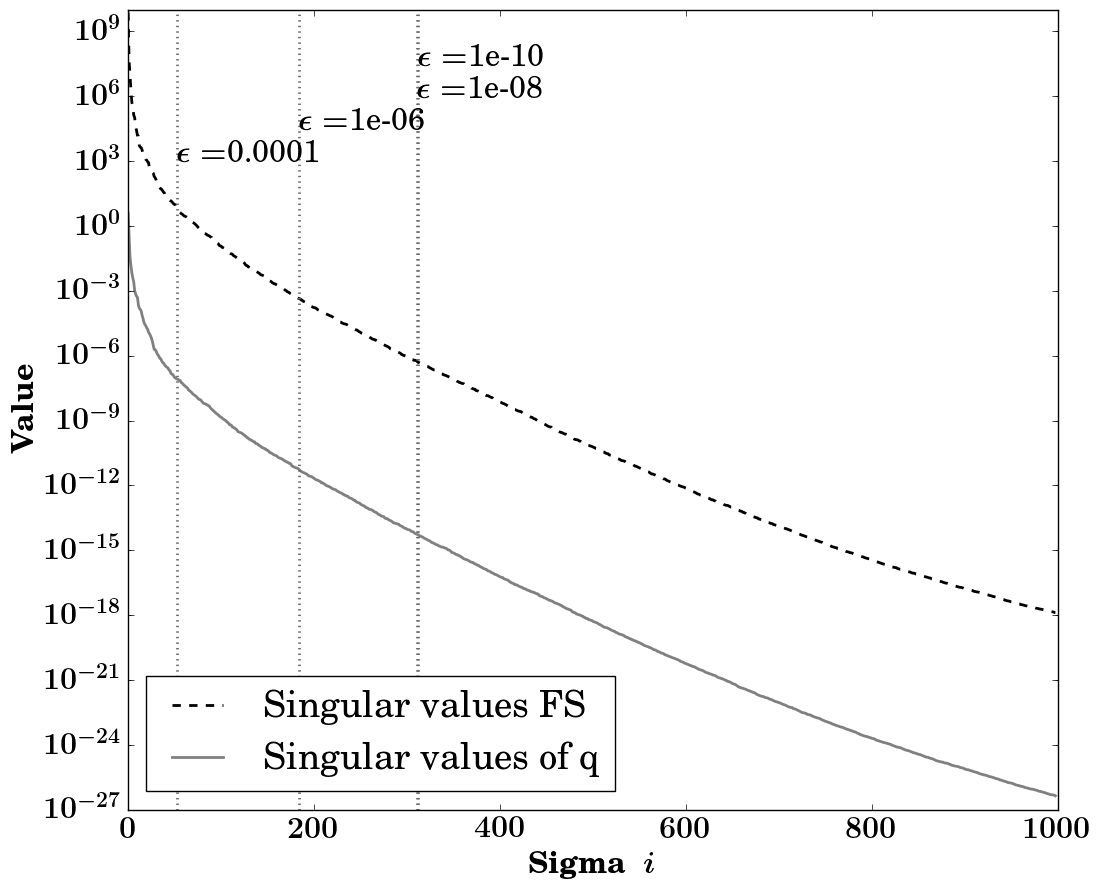
\includegraphics[width=0.6\textwidth]{singularvalues_full_trajectory.png}
  \caption{Distribution of singular values from a SVD of $12\_3000$, a matrix of snapshots distributed over the whole year.}
  \label{fig:singularvalues_full_trajectory}
\end{figure}

The first experiments were done with a one tracer model, the so called N-model
in Metos3D. To test and show the feasibility of the reduction a specific fixed parameter set $u_r =\{0.02,2.0,0.5,30.0,0.858\}$ was used to generate snapshots. These
parameters are taken from \cite{metos3dsimpack}, where they are given as the parameter set of a reference solution. A  uniformly distributed start concentration of $2.17\frac{mmol}{m^3}$ was used.
The time scale was set to $6000$ model years and three model states in each month were saved. The reason to only save three states out of the 2880 in one year, was the size of the data. One state vector used $0.422KB$ and two have to be save for each state, one for the full system and the other one for the nonlinear part. Thus, storing 2880 snapshots would have taken
$2.37GB$ per year.
Therefor, it was tried to reduced the amount of snapshots taken.
Different snapshot matrices were build from these saved states to try out how many must be taken to build an accurate reduced-order model (ROM). 

Figure \ref{fig:singularvalues_full_trajectory} shows the distribution of the first 1000 singular values from an SVD of a snapshot matrix  $S = \{y^{i}_1,\ldots,y^{i}_{3000}\}$ for $i =1,\ldots,12$ (called $12\_3000$). These snapshots are distributed uniformly over
the whole year and are taken at the end of each month, thus $12 \times 3000 = 36000$ snapshots were taken. 
The solid line are the singular values of the nonlinear snapshots and the dashed line are the ones from the snapshots of the full system. 
These two behave very similar, independently from the choice of the snapshot distribution.
The vertical dotted lines point out the estimated dimension $k$ of the base with a POD error $\epsilon$, computed with \eqref{Chapter2:eq:error_funcion_pod}.
It shows that an $\epsilon < 10e-8$ does not change $k$ anymore. 

\begin{figure}[H]
\centering
  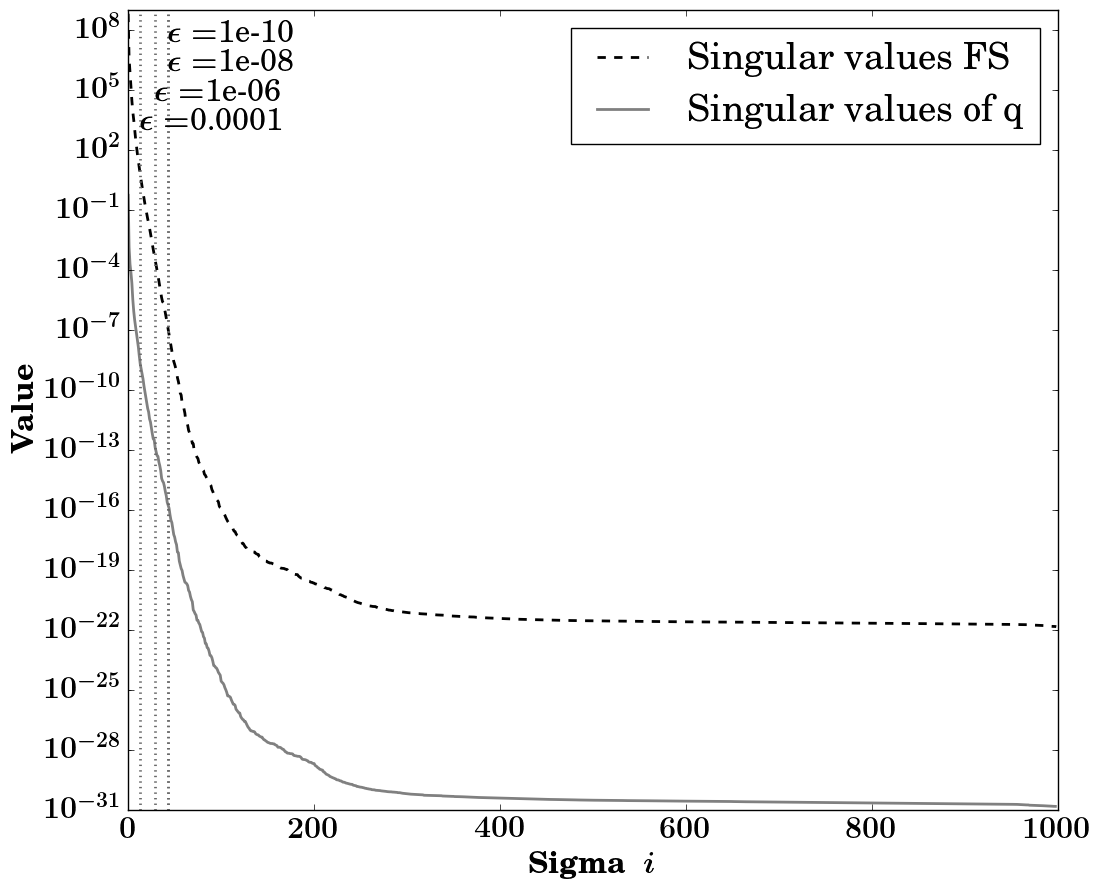
\includegraphics[width=0.6\textwidth]{singularvalues_one_month.png}
  \caption{Distribution of singular values from an SVD of $3\_3000$ a matrix of snapshots taken only in winter.}
  \label{fig:singularvalues_one_month}
\end{figure}

In comparison with Figure \ref{fig:singularvalues_one_month} the singular values descend slowly. There the singular values of an SVD from $S = \{y^{1}_1,y^{2}_1,y^{12}_1,\ldots,y^{1}_{3000},y^{2}_{3000},y^{12}_{3000} \}$  (called $3\_3000$)
are plotted. In the literature \cite[][p. 261]{ROM_Book} it is written that fast decaying singular values are a requirement for constructing efficient ROMs and
are an indicator for the quality of the ROM.


The snapshots for the singular values in Figure \ref{fig:singularvalues_one_month} were taken only in winter. The distribution seems to be more feasible for a ROM, but since
only data in winter time were taken into account, the ROM resulting from the corresponding singular vectors is inaccurate in summer time, as shown in Figure \ref{fig:error_one_month}. 
It shows that at least one snapshot in each month has to be used because otherwise the reduced model will leak accuracy in the months that are left out. There the relative error
\begin{equation}\label{eq:relativeError}
 \mathcal{E} = \parallel y^{FO}_j - y^{RO}_j \parallel_2/ \parallel y^{FO}_j \parallel_2
\end{equation}
over the period of a whole year from two different bases is plotted. The one, where only snapshots in winter
time contributed to the base, (dashed line) has an increasing error in summer time, which leads to a drifting of the solution. The other one (dotted line), where the snapshots were distributed over the whole year, is more accurate and has nearly the same error over the course of the entire year.

\begin{figure}[H]
\centering
  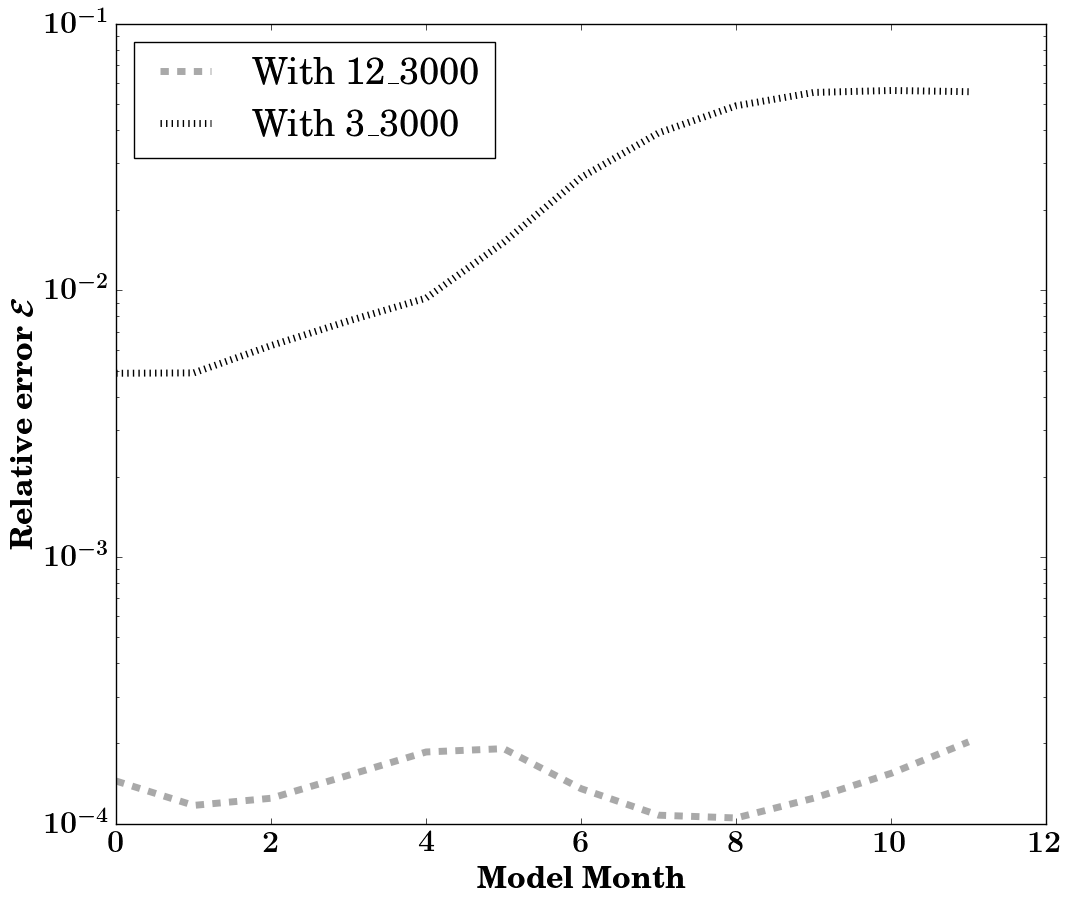
\includegraphics[width=0.6\textwidth]{relative_error_one_month.png}
  \caption[Relative error $\mathcal{E}$ during the course of a year for two different bases.]{Relative error $\mathcal{E}$ during the course of a year for two different bases. One where the Snapshots where taken in winter only and the other with snapshots distributed over the whole year.}
  \label{fig:error_one_month}
\end{figure}
Comparing the plots of the different singular values in Figure \ref{fig:comparison_differnt_singuarvalues} with the relative error of the
derived ROMs in Figure \ref{fig:relative_error}, it is not possible to see the correlation of the quality of the ROM with the singular values as proposed in the literature.
Interesting is that the singular values of $12\_3000$ and $12\_6000$ are very similar and the behavior of the derived ROMs is similar as well, 
as shown in Figure \ref{fig:spinup} and \ref{fig:relative_error}. This indicates that taking snapshots after 3000 model years into the snapshot set does not change the ROM.
Thus, it is sufficient to take only snapshots from the first 3000 model years, but it is better to take more snapshots during the course of the model years.

\begin{figure}[H]
\centering
\begin{subfigure}{.5\textwidth}
  \centering
  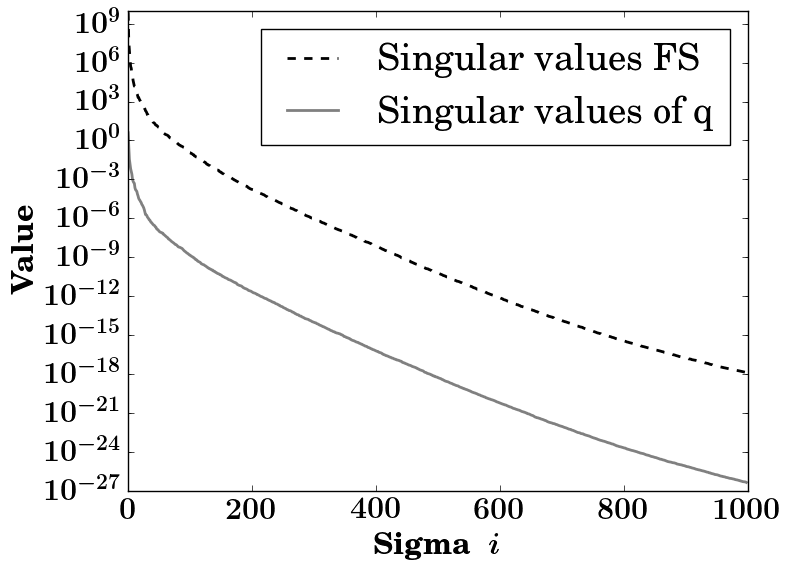
\includegraphics[width=1\textwidth]{singularvalues_12_3000.png}
  \caption{$12\_3000$}
  \label{fig:sing_sub1}
\end{subfigure}%
\begin{subfigure}{.5\textwidth}
  \centering
  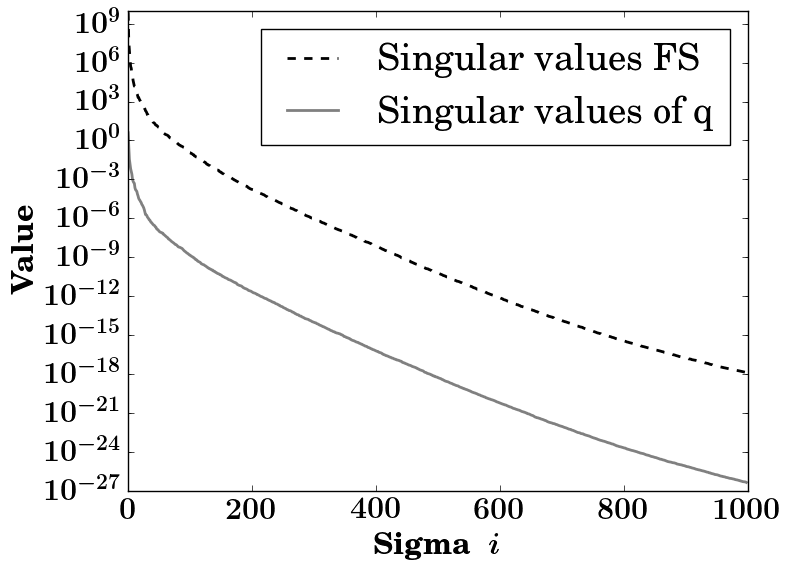
\includegraphics[width=1\textwidth]{singularvalues_12_6000.png}
  \caption{$12\_6000$}
  \label{fig:sing_sub2}
\end{subfigure}
\begin{subfigure}{.5\textwidth}
  \centering
  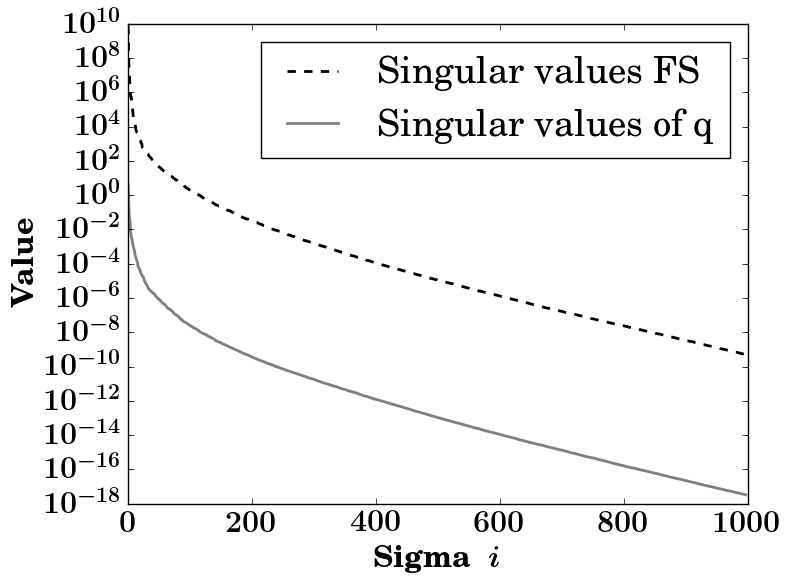
\includegraphics[width=1\textwidth]{singularvalues_36_1000.png}
  \caption{$36\_1000$}
  \label{fig:sing_sub3}
\end{subfigure}%
\begin{subfigure}{.5\textwidth}
  \centering
  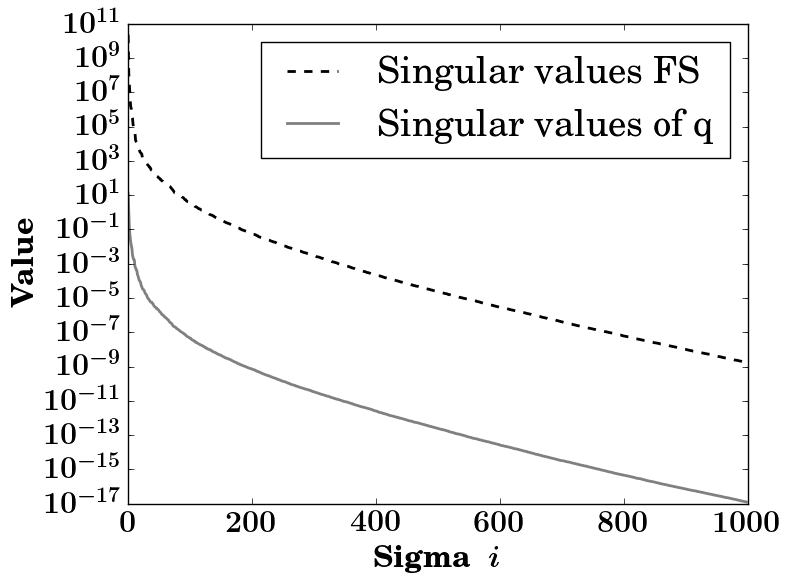
\includegraphics[width=1\textwidth]{singularvalues_36_3000.png}
  \caption{$36\_3000$}
  \label{fig:sing_sub4}
\end{subfigure}
\caption{Distribution of singular values from an SVD of different snapshot matrices.}
\label{fig:comparison_differnt_singuarvalues}
\end{figure}






\subsection{Approximation error and CPU time}\label{approxerrocputime}
To find out how to choose the dimension of the POD and the DEIM basis, a row of experiments were made. The singular vectors for these bases come from the SVD of uniformly distributed snapshots over 3000 model years ($12\_3000$), see Figure \ref{fig:singularvalues_full_trajectory}
for the corresponding singular values. In these experiments the size of one base was fixed and the size of the other one was changed. The size of a base marks the number of left singular vectors of the SVD that are taken to build the base. 
In Figure \ref{fig:comparison_differnt_pod_diem}
the behavior of the average relative error 
\begin{equation}\label{arerror}
\bar{\mathcal{E}} = \frac{1}{n_t} \sum\limits_{j=0}^{n_t}{ \parallel y^{FO}_j - y^{RO}_j \parallel_2/ \parallel y^{FO}_j \parallel_2}
\end{equation}
with $n_t = 1000$ is shown on the left. Either the DEIM dimension is fixed (black with dots) at $m=150$ or the POD dimension $k=150$ is fixed (gray with diamonds). It can be seen that both lines are limited to
the same accuracy and also the error of a ROM with both bases dimension of $300$ (gray star) does not lead to a better
approximation. The fixed POD ROMs reach that point as the dimension of the DEIM base is larger than $40$. Below that the approximation
gets worse. The fixed DEIM ROMs converge slower at a POD base size of $130$. Thus, chose the size of the POD base around $
130$ and the DEIM base around $40$ could be sufficient for the accuracy of the ROM. Note that, in this case, only information from the first 1000 model years are used and for longer model runs this might change.

\begin{figure}[H]
\centering
\begin{subfigure}{.5\textwidth}
  \centering
  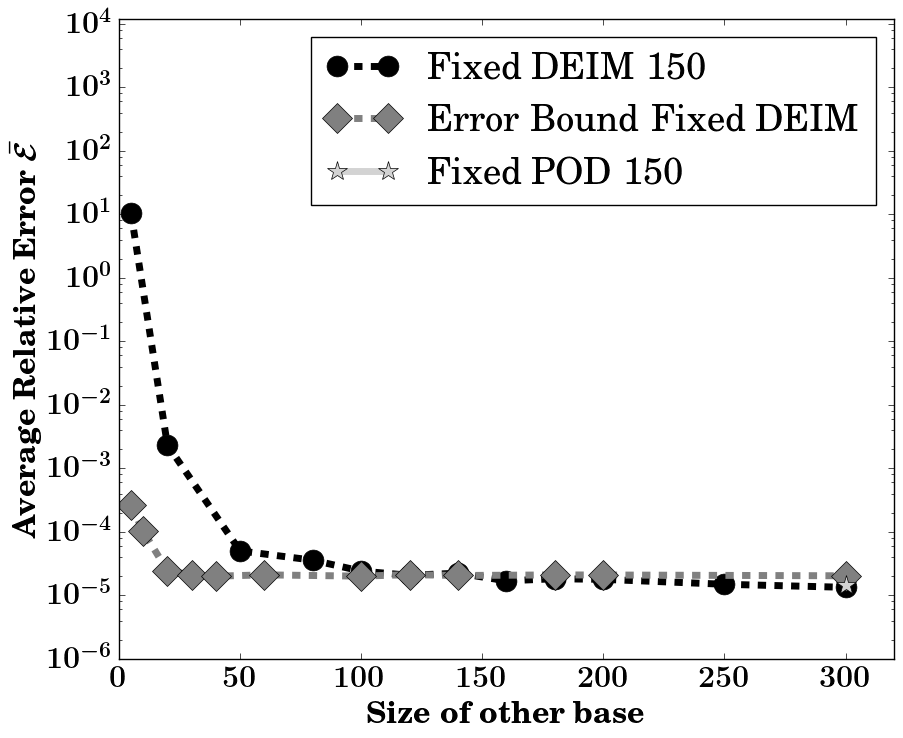
\includegraphics[width=1\textwidth]{realative_error.png}
  \caption{Relative error}
  \label{fig:compare_sub1}
\end{subfigure}%
\begin{subfigure}{.5\textwidth}
  \centering
  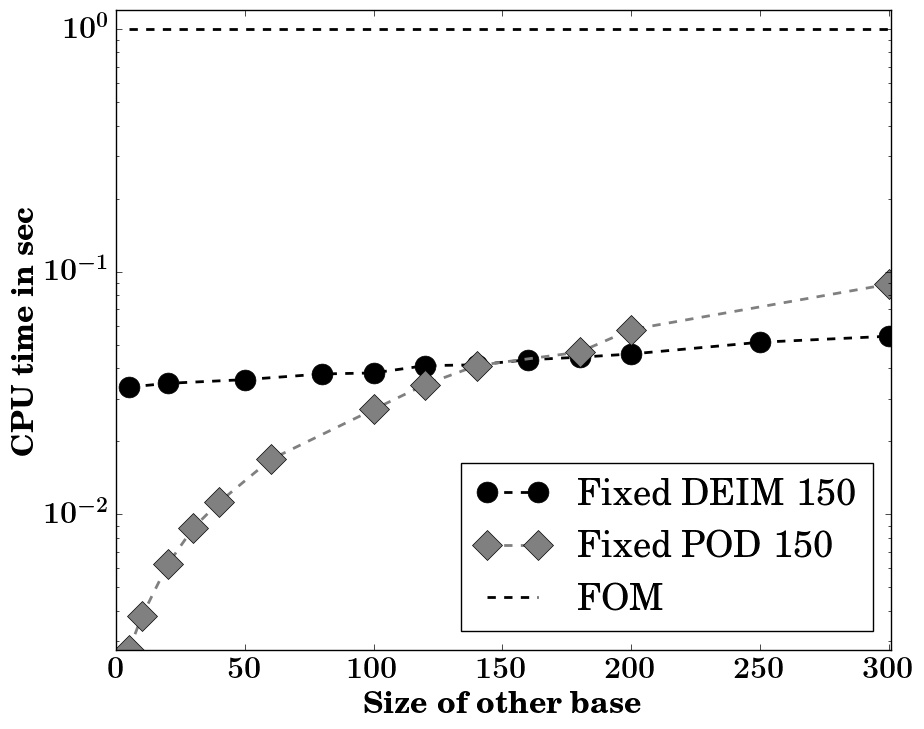
\includegraphics[width=1\textwidth]{avarage_cpu_time.png}
  \caption{Average scaled CPU time}
  \label{fig:compare_sub2}
\end{subfigure}
\caption[The average relative error and the average CPU time of different ROMs of the N-Model.]{The average relative error \eqref{arerror} of different ROMs is shown on the left side and average CPU time for these ROMs on the right.}
\label{fig:comparison_differnt_pod_diem}
\end{figure}


On the right side of Figure \ref{fig:comparison_differnt_pod_diem} the average CPU time for one model year of these ROMs with different base sizes is shown. The CPU time was taken over 1000 model years and scaled with the time of the 
full-order model (FOM). The black line with dots, where the size of the POD base changes, indicates that a large POD base does not lead to 
a strong increment of CPU time for the whole system. whereas changing the size of the DEIM base leads to a noticeable change in CPU time, as shown by the gray line with diamonds. This was made with
a one tracer model and will change with more tracers since the amount of matrix vector multiplications in \eqref{metos_red} will grow linear with the number of tracers. 
Overall a speed up between $10$ and $100$ is possible. For the minimal size of the bases, derived from the left side in Figure \ref{fig:comparison_differnt_pod_diem},
the speed up would be close to $100$. 
In Figure \ref{fig:error_bound} the real average relative error of the bases is compared to the approximated error bound of the POD-DEIM approach from Chapter \ref{Chapter2}.
The bounds are quite pessimistic, but they show a similar behavior as the real error, if the base size changes. There it is even better to see that the error of the POD part is
governing the error of the whole system. 
\begin{figure}[H]
\centering
  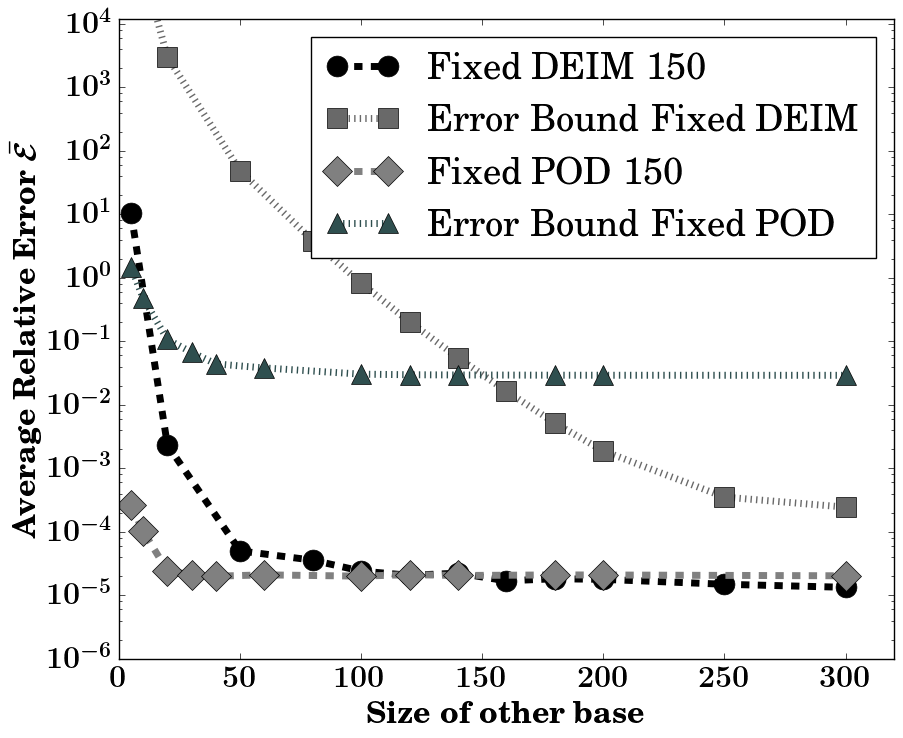
\includegraphics[width=0.7\textwidth]{realative_error_bound.png}
  \caption{The average relative error $\bar{\mathcal{E}}$ compared to the error bounds \eqref{ch2:error_bound_pod},\eqref{ch2:error_bound_deim} of the POD-DEIM approach.}
  \label{fig:error_bound}
\end{figure}
In conclusion, increasing the DEIM base size over the size of the POD base does not lead to a better approximation, but this increases the CPU time a lot. The increase of size of the POD base over the size of the DEIM instead does lead to a
decreasing approximation error. Therefore, the size of the POD base should be chosen larger than the size of the DEIM base or 
at least they should have the same size.

\subsection{Behavior of the Reduced-Order Models}\label{behaviorofroms}

In order to explore the convergence and the error behavior of different bases long simulations were made. 
The base names begin with the name of the SVD, i.e. $12\_3000$, which means 12 snapshots per year and 3000 years of data. Then follows a pattern like $P100D50$, where $P100$ means a POD basis of dimension $k=100$ and $D50$ means a DEIM basis of dimension  $m=50$.
At first, the convergence towards a periodic steady state was tested and compared to the convergence behavior of the full-order model.
In Figure \ref{fig:spinup} the spin-up norm 
\begin{equation}\label{eq:spinupnorm}
 S_{norm} = \parallel y_l - y_{l-1} \parallel_2 
\end{equation}
is plotted, which is the norm of the difference between the initial states of consecutive model years $l$.
It shows that none of the ROMs reaches a periodic steady state.
The full-order model reaches a periodic steady state after about 7000 model years, as shown in Figure 2 in \cite{metos3dsimpack}.


\begin{figure}[H]
\centering
  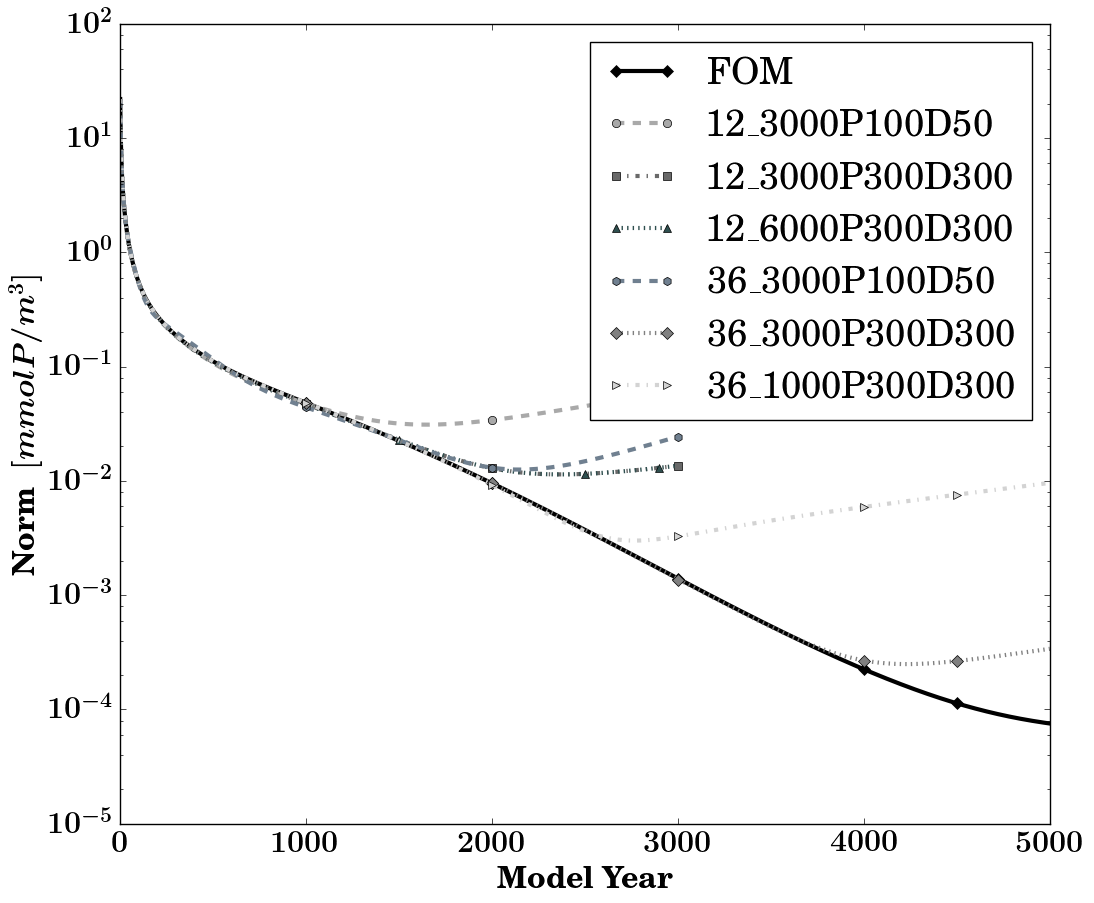
\includegraphics[width=0.8\textwidth]{spinupnorm_base_compare_2.png}
  \caption{Spin-up norm of different reduced-order models in comparison with the spin-up norm of the full-order model.}
  \label{fig:spinup}
\end{figure}
All ROMs diverge at some point. The ROM out of $12\_3000P100D50$ starts to deviate first, at about 1000 model years, form the black line, which
shows the spin-up behavior of the full-order model. The ROMs $12\_3000P300D300, 12\_6000P300D300$ and $36\_3000P100D50$ depart after 1500 model years and
begin to diverge. The ROM $36\_3000P100D50$ increases faster than the other two because of the smaller size of the bases. The ROM derived 
from the longer timeline of snapshots behaves in the same way as the base that is derived from only snapshots out of 3000 model years.
The ROM $36\_3000P300D300$ is the last one that departs from the behavior of the FOM, after about 3800 model years. This is far away from the other ones which show similar behavior.  
The ROM derived from only snapshots of 1000 model years diverges at around 2500 model years, this is later than the $12\_3000P300D300$ ROM. This indicates again that taking more snapshots during the year is more important than the total number of years 
that are taken into account.


Figure \ref{fig:relative_error} shows the relative error \eqref{eq:relativeError} of the same bases. The error was measured over 3000 model years and was computed the end of each year.
All ROMs show an increasing error over the 3000 years. Again the ROMs $12\_3000P300D300$ and $12\_6000P300D300$ show a similar behavior and the ROM out of $12\_3000P100D50$ has the largest error and the fastest increase.


\begin{figure}[H]
\centering
  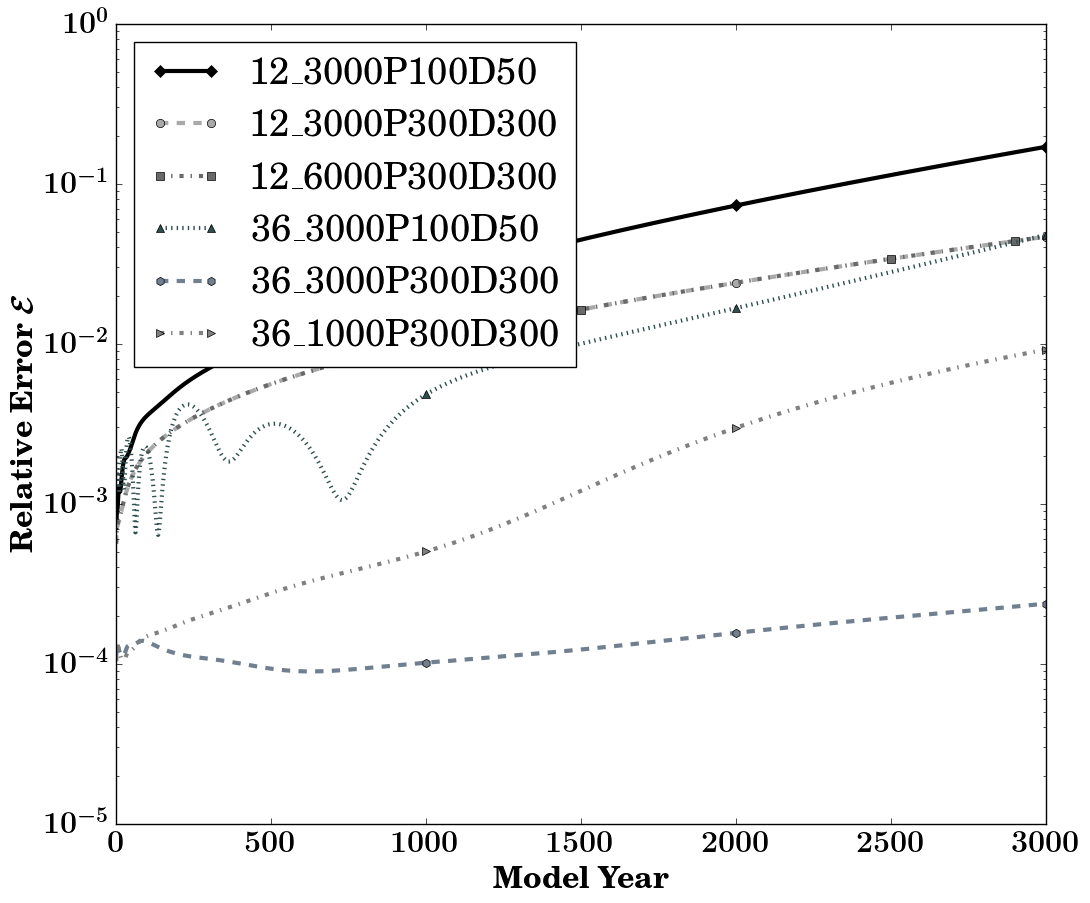
\includegraphics[width=0.8\textwidth]{error_norm_base_compare_2.png}
  \caption{Relative error $\mathcal{E}$ of different reduced-order models.}
  \label{fig:relative_error}
\end{figure}

The error of all ROMs oscillates at the beginning, usually only the first 100 model years, but the error of $36\_3000P100D50$ has a strong oscillation until 1000 model years.
Afterwards, it shows the same increase as the black line of $12\_3000P100D50$. The ROM $36\_3000P300D300$ shows the slowest error increment as well as a
very different behavior in the first 500 model years. At first, it oscillates as well, but only a couple of model years, after that it slightly decreases until around 600 model years.
Then the increment starts, but it is much slower than that of the other ROMs. The base $36\_1000P300D300$, where only snapshots from the first 1000 model years were taken, starts 
with the same error as $36\_3000P300D300$, but shows a stronger increment over the model years.

In conclusion, large bases have a better convergence behavior and a smaller approximation error. Taking snapshots throughout a longer time period than 3000 model years does not change the convergence behavior nor the relative error. Indeed, changing the amount of snapshots per year influences both.


To show some more quantities of the ROMs, four bases have been picked out and compared in Table \ref{Chapter4:table}.
The bases are generated out of two different snapshot sets, one is the set $36\_3000$, the other is the set $36\_1000$.
For each of them two bases are selected with different POD and DEIM base sizes.
For each of them the following quantities have been measured:
\begin{itemize}
 \item $t_{setup}$ - The time which is required to pre-compute the SVD, the DEIM indices and the matrices $A_{ri}$ and $P_{ri}$. Note that this only has to be performed once. 
 The SVD was computed with SLEPc on an Intel\textsuperscript{\textregistered} Sandy Bridge EP architecture with Intel Xeon\textsuperscript{\textregistered}  E5-4640 that consist of 8 cores running at 2.4 GHz. The DEIM indices and the base matrices with 
 Intel Core\textsuperscript{\textregistered} i7-4750HQ that consist of 8 cores running at 2 GHz. They where computed sequentially and the SVD was computed with 96 cores in parallel.
 \item $S_P$ - The speed up for a model year, which is the ratio of the computational time for a model year of the FOM and the ROM. They were both computed sequentially on the i7-4750HQ.
 \item $M_{a}$ - The relative mass change of the model after $a$ years, scaled with the total mass of the tracer at $t=0$, i.e. $\frac{\parallel V_{y_a} \parallel_1 - \parallel V_{y_0} \parallel_1}{\parallel V_{y_0} \parallel_1}$, where $V_{y_a}$ is a vector 
 of the masses of the tracer $y_a$. 
 \item $\bar{\mathcal{E}}_{a}$ - The average relative error \eqref{arerror} over $a$ years. 
 \item $\bar{\mathcal{E}}_{*}$ - The approximated error bound of the POD-DEIM approach as defined in Chapter \ref{Chapter2}. 
 \item $R_{a}$ - The number of spin-ups (model years) that the FOM needs to get to the solution of 3000 model years, if initialized with the output of the ROM at model year $a$. 
\end{itemize}

\begin{table}[H]
\begin{center} 


$\begin{array}{|l|c|c|c|c|c|}
\hline
\text{SVD} & \multicolumn{2}{c|}{36\_3000} & \multicolumn{2}{c|}{36\_1000} & - \\
\hline
\text{Base}  & P100D50 & P300D300  & P100D50 & P300D300  & FOM\\
\hline t_{setup} [s]  & (9676,10,39) & (9676,870,327) & (2071,9,38) & (2071,989,350) & -\\

\hline S_P  & 78.29 & 7.35  & 73.00 & 9.08 & -\\

\hline M_{1000}  & 0.00227 & 0.00019  & 0.00102 & 0.00056 & 0.00013\\

\hline M_{3000}  & 0.03727 & 0.00056  & 0.25539 & 0.00725 & 0.00039\\

\hline \bar{\mathcal{E}}_{1000}  & 0.00252 & 0.00010  & 0.00156 & 0.00029 & -\\

\hline \bar{\mathcal{E}}_{3000}  & 0.01409 & 0.00014  & 0.06661 & 0.00250 & -\\

\hline \bar{\mathcal{E}}_{*}  & 77.35 & 0.11475  & 44.72 & 0.05972 & -\\

\hline R_{1000}  & 2028 & 1995  & 2114 & 1996 & -\\

\hline R_{3000}  & 1711 & 40  & 2755 & 758 & -\\
\hline
\end{array}$
\end{center}
\caption{Comparison of four ROMs from the N-Model}
 \label{Chapter4:table}
\end{table}
The time to set up the ROMs is dominated by the computation of the SVD, which is only possible because only a truncated SVD was computed in parallel.
In the 9676 seconds (2.6h)  and 2071 seconds (0.57h) two SVDs were computed, one for the POD method and one for DEIM. The time
to compute the DEIM indices grows fast with the size of the DEIM base because of the complexity of the Algorithm \ref{Chapter2:deim_algorithm}.

The relative mass change for the $P100D50$ ROMs is much higher than that of the $P300D300$. 
It is increasing from 1000 to 3000 model years for all of the ROMs.
The $36\_3000P300D300$ has nearly the same mass change as the FOM. 
The average relative error is increasing a lot from 1000 to 3000 model years, except for the $36\_3000P300D300$ ROM. The approximated error bound $\bar{\mathcal{E}}_{*}$ is not accurate and roughly three orders of magnitude away from the 
real error. It indicates that the $36\_1000$ ROMs should be more accurate than the $36\_3000$ ROMs. This is due to the fact that the smaller snapshot matrix has smaller singular values and the approximated error bound relies mostly 
on the singular values.

If the output solution of one of the ROMs after 1000 model years were taken and the FOM is initialized with them, the FOM needs nearly the rest of the 3000 model years to
get to the original solution. If the output of the ROMs after 3000 model years is taken only the ROM $36\_3000P300D300$ supplies a solution that is
near the one after 3000 model years of the FOM. The other are far away, even further away as the solution at 1000 model years as for the
ROM $36\_1000P100D50$, which takes 2755 model years in the FOM. If it is done like this, i.e. combining one ROM with the FOM, all the systems will give an overall speed up of approximated 1.4, if supplied with the ROM solution of 1000 model years.
The system supplied with the solution after 3000 model years of the ROM $36\_3000P300D300$ will only need time equivalent to $\frac{3000}{7.35}  + 40 = 447$ model years of the FOM to get to the original solution of 3000 model years.
This leads to an overall speed up of $\frac{3000}{447} \approx 6.71$.
Note that here CPU times of different implementations are compared, the FOM is implemented in C with PETSc and the ROM is implemented in python with numpy and both were run sequentially.
It is expected to get a better speed up if the ROM will be implemented in C as well.

In conclusion, the creation of a reduced-order model of the N-Model is feasible and the POD-DEIM leads to an adequate reduction in
computational cost. As long as the snapshots and reduced matrices only have to be computed once and then the reduced system is solved
many times with them. This leads to the question whether it is possible using one reduced model for different sets of parameters and get accurate solutions.
This problem will be described in Chapter \ref{Chapter5}. In the next chapter the reduction of a two tracer model is explained and
the results of experiments with it are presented.




\section{Experiments with N-DOP-Model}\label{numerical_n-dop}
The model used in these experiments uses two tracer elements. It extends the N-model, which considers only inorganic phosphate ($PO_4$ called $N$ here) with dissolved
organic phosphorus (called DOP). All uptake of phosphate is shifted either to export production or to DOP in this model. It is further described in
\cite{biomodels}. The model uses one vector for each tracer, and thus, there are two solution vectors.
36 uniformly distributed snapshots per year from the first 1000 model years were generated. For this the parameter set $u= \{0.02,2.0,0.5,30.0,0.67,0.5,0.858\}$  was used and the start concentration was set to $2.17\frac{mmol}{m^3}$ and $1e^{-4} \frac{mmol}{m^3}$, for N and DOP respectively.
There are two strategies how to create a ROM for this model, one is to create one snapshot matrix out of the combined tracers vectors, i.e. 
\begin{equation*}
S = \left [
\begin{array}{ccc}
\vertbar &        & \vertbar \\
 y^N_1 &  \ldots & y^N_{ns}\\
 \vertbar &        & \vertbar \\
  \vertbar &        & \vertbar \\
 y^{DOP}_1 & \ldots& y^{DOP}_{ns}\\
 \vertbar &         & \vertbar \\
\end{array} \right ].
\end{equation*}
The other option would be to create two independent matrices 
\begin{equation*}
S_N = \left [
\begin{array}{ccc}
 y^N_1 &  \ldots & y^N_{ns}\\
\end{array} \right ], \quad
 S_{DOP} = \left [
\begin{array}{ccc}

 y^{DOP}_1 & \ldots& y^{DOP}_{ns}\\

\end{array} \right ]
\end{equation*}
and create one POD-DEIM base for each tracer. 
The first one has not lead to a usable ROM because the DOP solution vector was tremendously inaccurate. A possible reason might be the fact that the DEIM algorithm has picked out indices only in the upper part of the combined vector, thus, in the $y^N$ part.
Consequently, for the nonlinear part only information from the solution of one tracer were taken into account. Thus, the part of other tracer were only bad approximated.

In the following, the results of the second, decoupled approach are presented. Therefore, a matrix with 36 equally distributed snapshots for each model year over 1000 model years was created and the 
SVD was computed. The singular values of both tracers in Figure \ref{fig:singularvalues_N-DOP} look similar to those from the N-Model. Thus, it is expected that the resulting ROM will give similar results as well.

\begin{figure}[H]
\begin{subfigure}{.48\textwidth}
  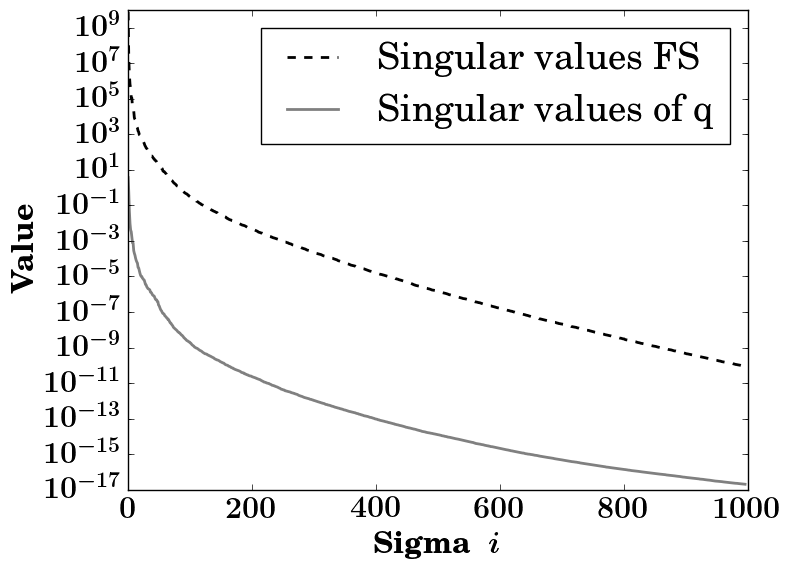
\includegraphics[width=1\textwidth]{singularvalues_N-DOP_1000_N.png}
  \caption{Singular values of $S_N$}
  \label{fig:sing_N-DOP_sub1}
\end{subfigure}%
\begin{subfigure}{.5\textwidth}
  \centering
  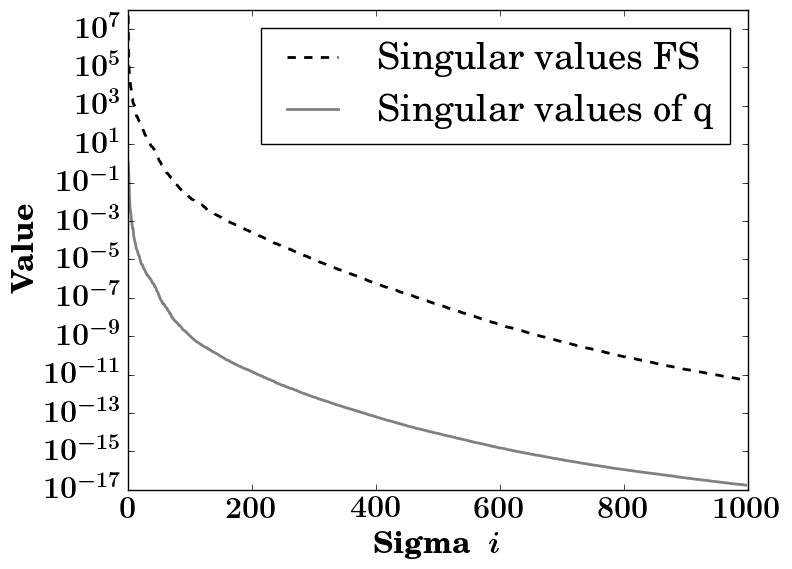
\includegraphics[width=1\textwidth]{singularvalues_N-DOP_1000_DOP.png}
  \caption{Singular values of $S_{DOP}$}
  \label{fig:sing_N-DOP_sub2}
\end{subfigure}
\caption{Distribution of the singular values of 36\_1000 from the N-DOP-Model.}
\label{fig:singularvalues_N-DOP}
\end{figure}

In Figure \ref{fig:spinup_N-DOP} the spin-up norm \eqref{eq:spinupnorm} of two ROMs of the N-DOP-Model is shown for each tracers. 
The ROM with the smaller base matrices shows a very different spin-up behavior than the FOM. Both tracer concentrations
are oscillating during the first 500 model years. 
\begin{figure}[ht]
\centering
  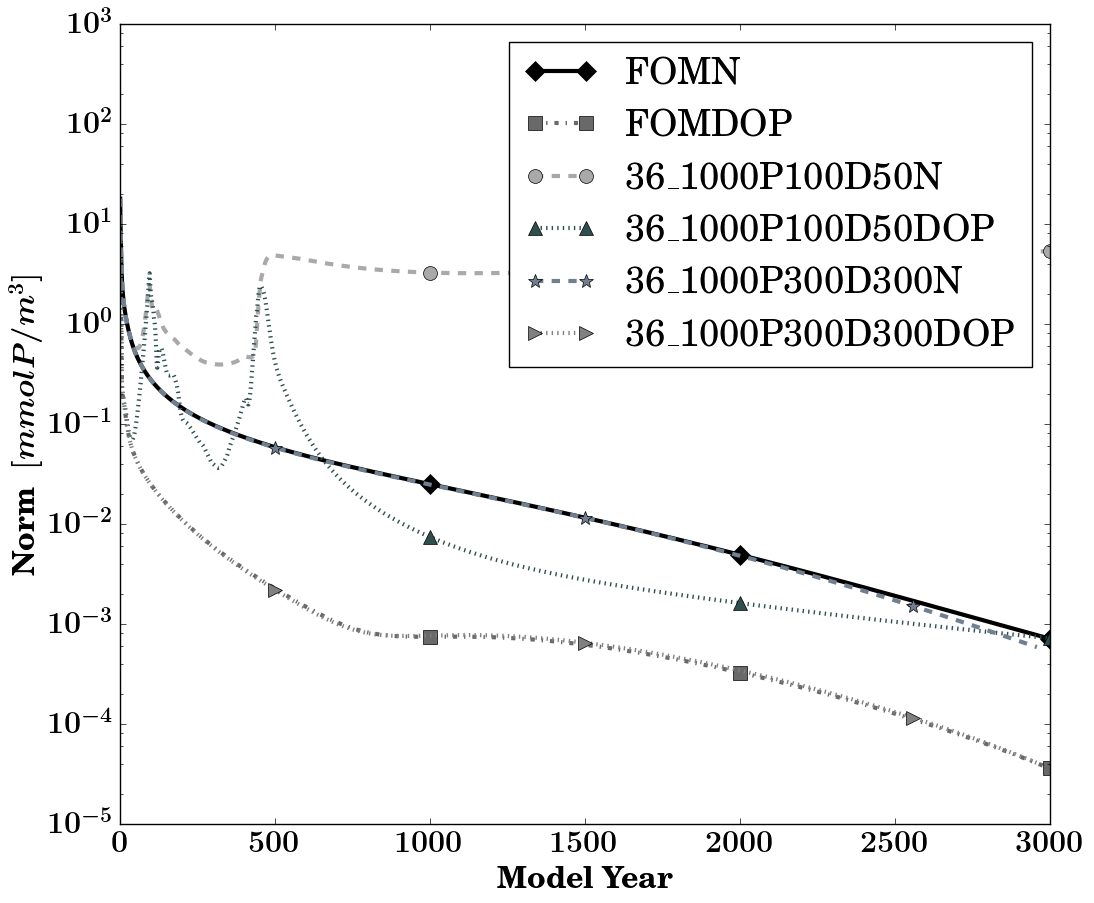
\includegraphics[width=0.8\textwidth]{spinupnorm_base_compare_N-DOP.png}
  \caption{Spin-up norm of two ROMs in comparison with the spin-up norm of the FOM of N-DOP.}
  \label{fig:spinup_N-DOP}
\end{figure}
Afterwards, the N concentration is changing a lot from model year to model year, but the change
does not increase. The DOP concentration converges to a state with only small changes each model year.
The other ROM, that is shown in Figure \ref{fig:spinup_N-DOP}, has nearly the same change of concentration over the 3000 model years as the FOM. This is interesting because
the ROM was only created with information of the first 1000 model years and such a ROM of the N-Model diverges stronger from the FOM, compare Figure \ref{fig:spinup}.

The relative error \eqref{eq:relativeError} over 3000 model years for each tracer of these ROMs is presented in Figure \ref{fig:relative_error_N-DOP}.
First of all, note that in this case it relates to a relative error and values higher than one mean that the error is larger than the 
2-norm of the original solution vector of the FOM. Thus, the error of both concentrations (N,DOP) of the smaller ROM is large compared to 
the overall concentration in the FOM, and the N part shows a strong increasing over the model years. The DOP part is nearly constant after one peak at about 500 model years.
Since the relative error of the ROM $36\_1000P100D50$ increases far beyond one after 500 model years, 
the solution of this ROM is not close to the solution of the FOM.
\begin{figure}[ht]
\centering
  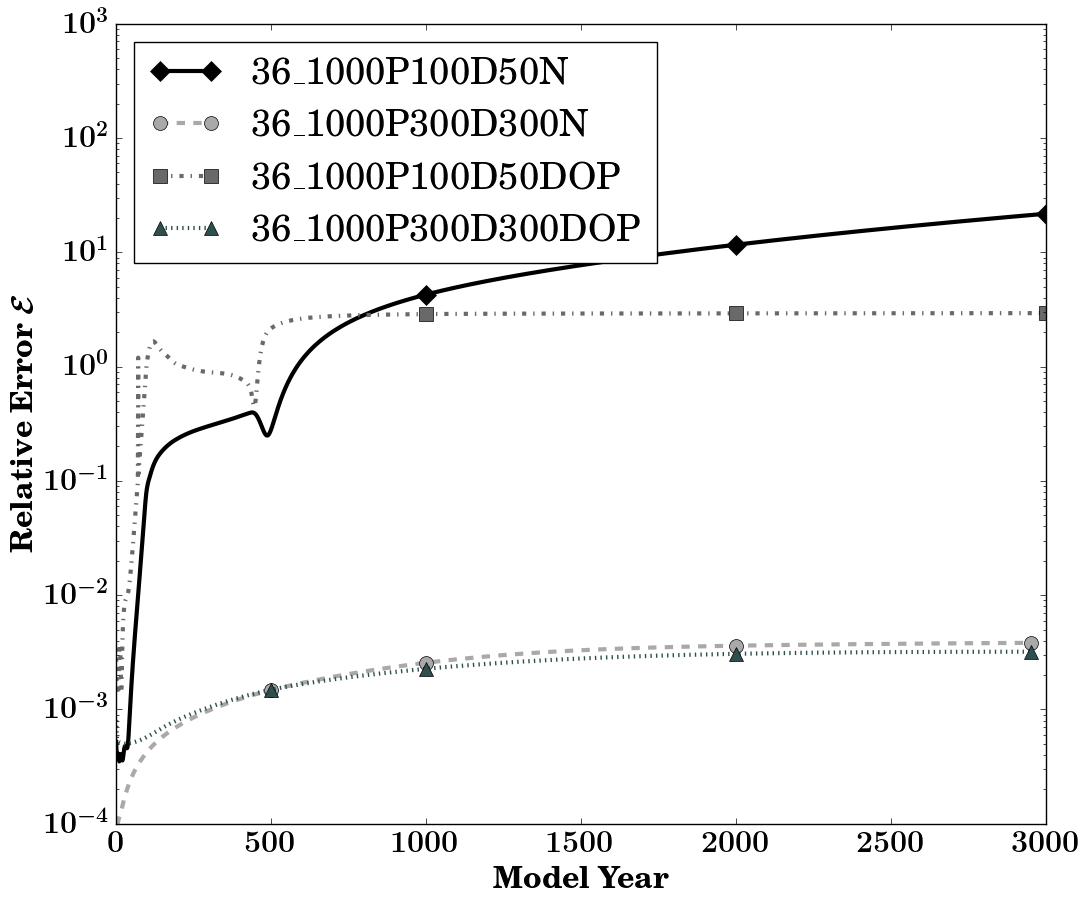
\includegraphics[width=0.8\textwidth]{error_norm_N-DOP.png}
  \caption{Relative error $\mathcal{E}$ of two ROMs of the N-DOP-Model.}
  \label{fig:relative_error_N-DOP}
\end{figure}
The relative errors of both concentrations of the 
ROM $36\_1000P300D300$ are increasing over the 3000 model years, at first, stronger and later they stay nearly constant. 
The are both very similar in each model year and in an order of $10^{-3}$.

Table \ref{Chapter4:table-N-DOP}
shows the same information as Table \ref{Chapter4:table} for the N-DOP-Model. The setup times of the 
ROMs are roughly doubled because each tracer has its own bases, and thus, its own setup process. Due to this fact the speed up is much smaller as well.
Since each tracer has its own and mostly different DEIM indices, the biogeochemical model has to be evaluated 
nearly twice the number of DEIM indices. In the ROM $36\_1000P300D300$ only 52 DEIM indices of the two tracers were identical, this is less then 10\%.
In addition, the number of matrices that must be interpolated is doubled as well because each tracer has its own
POD base. For a comparison of the CPU time of the main operations during one time step of the N-Model and the 
N-DOP-Model look in Appendix \ref{Appendix:cpupie}.

The relative mass change in the DOP concentration is tremendously high in all models as well as in the FOM, but the mass change of the ROM $36\_1000P300D300$ is nearly equal to that of the FOM. 
Note that the start concentration of DOP is $1e^{-4} \frac{mmol}{m^3}$, and thus, it has a really low amount of substance compared to the start concentration of N.
The N part of the model $36\_1000P300D300$ has less mass change than the FOM. This mass change becomes
even smaller after 3000 model years than after 1000, although, the mass change usually increases over the course of the model years.

The relative error of the ROM $36\_1000P100D50$ is higher than one as well after 1000 as after 3000 model years and for both tracers.
Supplying the solution of this ROM into the FOM, it does not come near the the original solution of 3000 model years within the
time of 3000 model years. Basically this results because of the poor approximation of the ROM, the resulting high relative mass change of the system, as well as the occurrence of
a lot negative concentration values. For DOP$\approx 75 \%$ and for N$\approx 1\%$ compared to approximately  $47\%$ and $0\%$ negative values in the solution of the
FOM after 3000 model years. The approximated error bounds for the ROMs are much closer to the actual error than in the N-Model.
The approximated error bound for the DOP tracer is lower than the actual error in both ROMs.
Since the tracers interact with each other, it is a question that has to be answered, whether the error bound of each tracer gives information about the error of the whole system.

The error of the ROM $36\_1000P300D300$ is similar in both tracers, and it is comparable to the error of the 
same sized ROM of the N-Model. The solution of this model is usable to produce a solution with the FOM that is close to the original solution. 
The FOM takes 2011 and 495 spin-ups to get to the original solution and with this setup a speed up of 1.7 is possible. This is less than the speed up of the
N-Model which depends mostly on the fact that a separate POD-DEIM base is used for each tracer.  
Overall, the POD-DEIM approach can be applied to the N-DOP-Model and the other multi tracer models, if a separate POD-DEIM base is used for each tracer.

\begin{table}[H]
\begin{center} 


 $\begin{array}{|l|c|c|c|c|c|c|}
 \hline
 
\text{Base}  & \multicolumn{2}{c|}{36\_1000P100D50} & \multicolumn{2}{c|}{36\_1000P300D300} & \multicolumn{2}{c|}{FOM}\\
\hline t_{setup} [s]  & \multicolumn{2}{c|}{3965,19,69} &\multicolumn{2}{c|}{3965,1989,646} & \multicolumn{2}{c|}{-}\\
\hline S_P  & \multicolumn{2}{c|}{14.47323} & \multicolumn{2}{c|}{2.42209}  & \multicolumn{2}{c|}{-} \\
\hline

\text{Tracer}  & N & DOP & N & DOP & N & DOP\\

\hline M_{1000}  & 2.607 & 1039.21  & 0.00652 & 184.282 & 0.00854 & 183.912\\

\hline M_{3000}  & 18.192 & 1073.76  & 0.00550 & 186.397 & 0.00874 & 185.631\\

\hline \bar{\mathcal{E}}_{1000}  & 1.293 & 1.803  & 0.00143 & 0.00142 & - & -\\

\hline \bar{\mathcal{E}}_{3000}  & 8.325 & 2.543  & 0.00279 & 0.00243 & - & -\\


\hline \bar{\mathcal{E}}_{*}  & 6.517 & 0.38633  & 0.00862 & 0.00044 & - & -\\

\hline R_{1000} &  \multicolumn{2}{c|}{-} &  \multicolumn{2}{c|}{2011} &  \multicolumn{2}{c|}{-} \\
\hline R_{3000} &  \multicolumn{2}{c|}{-} &  \multicolumn{2}{c|}{495} &  \multicolumn{2}{c|}{-} \\
\hline
\end{array}$


\end{center}
\caption{Comparison of two ROMs from the N-DOP-Model}
 \label{Chapter4:table-N-DOP}
\end{table}
In the next chapter the results of experiments with ROMs of the N-Model for parameter studies are presented.

%\section{Experiments with MITgcm-PO4-DOP-Model}
%\label{Chapter4:mitgcm}




